\documentclass[a4paper,12pt]{report}
\usepackage[left=2.0cm, right=2.0cm, top=2.0cm, bottom=2.0cm]{geometry}

\usepackage{setspace}
\usepackage{sectsty}
\usepackage{mathtools}
\usepackage{tkz-euclide}
\usetkzobj{all}
\doublespacing

\author{Matthew Webb}
\title{TorquePaper 2016.1: Accurate Shooter Tilt and Calculation}

\newcommand{\tab}{\hspace{20pt}}

\begin{document}
	\maketitle
	\tableofcontents
	
	\chapter{Calculating Tilt}
	\section{Initial Equation}
	
	\tab This equation was pulled from the Wikipedia article "Trajectory of a projectile", section called "Angle $\theta$ required to hit coordinate (x, y)". The derivation of this equation can be found on the Wiki page.
	\begin{center}
		\(\theta=\arctan{(\frac{v^2 \pm \sqrt{v^4 - g(gx^2 + 2yv^2)}}{gx})}\)
	\end{center}
	\tab By simply plugging in the velocity of the shooter, gravity, the distance between the robot and the tower (x), and the height from the top of the robot to the goal (y), the approximate angle $\theta$ can be calculated.
	\section{Problem}
	\tab The next problem is that when the shooter is tilted, the height of the robot - and thus the height between the top of the robot and the goal - changes. However, the required angle $\theta$ must be calculated before this modified height can be calculated. And in order to calculated the modified height, the angle is required. This sets up recursive equations, which cannot be solved. Therefore, a new equation must be derived.
	\section{Solution}
	\tab The solution to this recursive problem starts with defining the new modified height from given values. We start with the initial triangle where the top of the robot is at the bottom and the tower is across from it.
	\begin{center}
		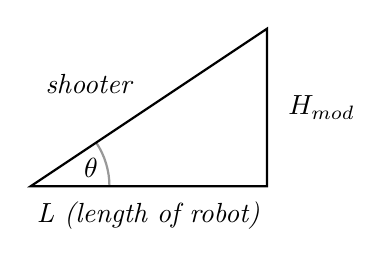
\begin{tikzpicture}[thick]
			\coordinate(A) at (0, 0);
			\coordinate(B) at (3, 0);
			\coordinate(C) at (3, 2);
			\draw (A)--(B)--(C)--cycle;
			
			\tkzLabelSegment[below=2pt](A,B){\textit{L (length of robot)}}
			\tkzLabelSegment[right=4pt](B,C){\textit{$H_{mod}$}}
			\tkzLabelSegment[above left=2pt](C,A){\textit{shooter}}
			
			\tkzMarkAngle[fill=orange,size=1cm,opacity=.4](B,A,C)
			\tkzLabelAngle[pos = 0.8](B,A,C){$\theta$}
		\end{tikzpicture}
	\end{center}
	\tab Using this equation, we can substitute in the first equation.
	\begin{center}
		\(H_{mod} = H - L * \frac{v^2 \pm \sqrt{v^4 - g(gx^2 + 2yv^2)}}{gx}\)
	\end{center}
\end{document}